\section{Capacitive Grading Techniques}
Capacitive graded bushings, sometimes referred to as the field stress-controlled bushing or capacitor bushing \cite{kuffel2000high}, contain concentric conductive foils within the insulation.
Each foil is isolated from the others \cite{Ahmed11}.
By designing the length and radial spacing of these foils, the electric stress and voltage drop in the core along its surface is determined by the ratio of partial capacitances between the foils \cite{Ahmed11}.
The difference between a standard solid bushing and a field stress-controlled bushing is shown in figure \ref{Figure:typesofbushing}.

\begin{figure}[!htb]
  \centering
  \subfigure[Solid Bushing]{
    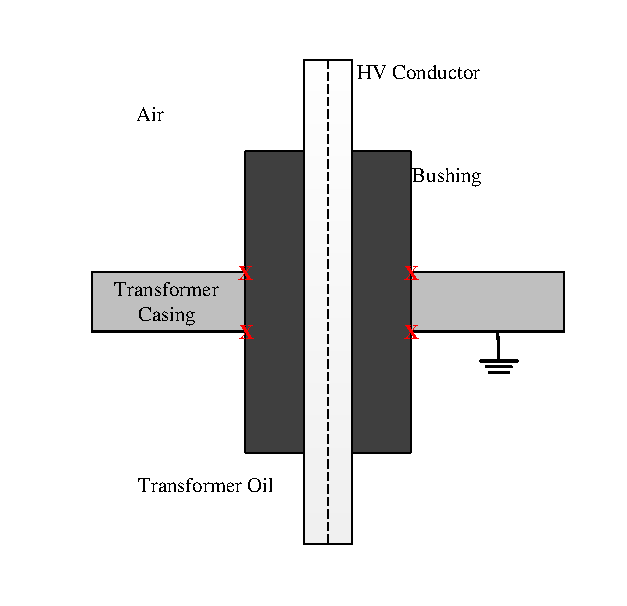
\includegraphics[height = 6cm]{GenericBushing.pdf} 
	\label{Figure:standardbush}
  }
  \subfigure[Field Stress-controlled Bushing]{
    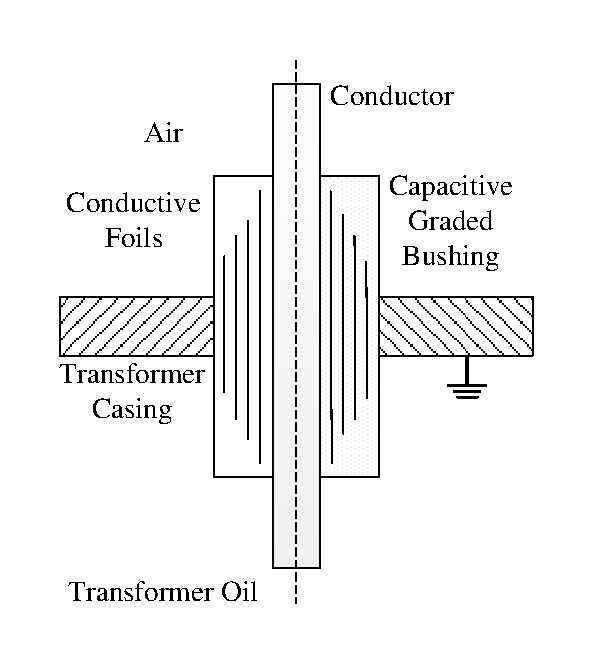
\includegraphics[height = 6cm]{GenericGradedBushing.pdf} 
	\label{Figure:gradedbush}
  }
\caption{This shows the difference in construction between the two bushing types}
  \label{Figure:typesofbushing}
\end{figure}



